%    Section: "Calculated permeabilities" (Yi, Nelson, Chris T.)
%      -the final, BEST logPs from each method at ~1-1.4 us each (Table 1)
%      -plots showing the comparison
%      -what are the errors?  (just numerically at this point)
%      -does increasing simulation time help?  (not really: case of urea)

\subsection*{Computed vs. experimental \perm}
  \par The computed log\perm~of the three permeants are listed in Table 1, along with the corresponding experimental references obtained from egg phosphatidylcholine bilayers (urea~\cite{Gallucci1971}, codeine~\cite{Orbach1980} and  benzoic acid~\cite{Walter1984}).
  % Egg lecithin and egg-PC are interchangeable. Both papers purchased egg-PC from avanti inc among other sources.
  From Table~1, it is clear that the majority of computed \perm~values exceed the corresponding experimental data by 1--2 orders of magnitude. For comparison, we define $\Delta$log\perm = log\permcom - log\permexp, where log\permcom~and log\permexp~are the computed and experimental log\perm, respectively. Negative $\Delta$log\perm~values are only observed for urea, the most hydrophilic of the three permeants.  Results obtained with different methods also show the largest discrepancy for urea: the US and REUS  methods underestimate log\perm~by 0.87 and 0.51, whereas ABF and MW-ABF overestimate it by 0.71 and 1.14, respectively. For benzoic acid and codeine, all the methods overestimate log\perm~by 0.71 to 1.67.

  %%\documentclass[11pt,letterpaper]{article}

%%\usepackage{color}

%%\setlength{\textwidth}{17cm}
%%\setlength{\textheight}{20.5cm}
%%\setlength{\oddsidemargin}{-.1cm}
%%\setlength{\topmargin}{-2 cm}

%%\renewcommand{\baselinestretch}{1.0}

%%\newcommand{\hl}[1]{\textcolor{red}{#1}}
\newcommand{\hl}[1]{\textbf{#1}}
\providecommand{\e}[1]{\ensuremath{\times 10^{#1}}}

%%\begin{document}

\begin{table}[h]
\centering
%\resizebox{\textwidth}{!}
{
\begin{tabular}{|c|c|c|c|}
\hline
 & Urea & Benzoic Acid & Codeine     \\ \hline 
%PAMPA  & \multicolumn{2}{c|}{-9.0}          & \multicolumn{2}{c|}{-3.94}                                                  & \multicolumn{2}{c|}{xx}        \\ \hline
% multiple columns probably too confusing - graph shows time dependence better anyway
% & \multicolumn{2}{c|}{Urea} & \multicolumn{2}{c|}{Benzoic Acid} & \multicolumn{2}{c|}{Codeine}      \\ \hline 
%Experiment & \multicolumn{2}{c|}{-5.4}          & \multicolumn{2}{c|}{-0.26}                                                  & \multicolumn{2}{c|}{-0.85}        \\ \hline
%US                & -5.97 (1.1\,$\mu$s)    & -6.27 (2.9\,$\mu$s)   & 0.35 (1.1\,$\mu$s)                         & 0.45 (1.4\,$\mu$s)                         & 0.08 (1.1\,$\mu$s)     & 0.03 (1.4\,$\mu$s)   \\ \hline
%RE-US              & -5.28 (1.1\,$\mu$s)    & -5.91 (4.3\,$\mu$s)   & 1.11 (1.1\,$\mu$s)                         & 1.17 (1.4\,$\mu$s)                         & 0.67 (1.1\,$\mu$s)     & 0.64 (1.4\,$\mu$s)   \\ \hline
%ABF               & \multicolumn{2}{c|}{-4.69 (0.9\,$\mu$s)} & \multicolumn{2}{c|}{1.16 (0.9\,$\mu$s)}                                           & 0.59 (1.1\,$\mu$s)     & 0.82 (2.7\,$\mu$s)   \\ \hline
Experiment & -5.4          & -0.26                                             & -0.85      \\ \hline
US                & -6.27 (2.8\,$\mu$s)   & 0.45 (1.4\,$\mu$s)             & 0.03 (1.4\,$\mu$s)   \\ \hline
REUS              &  -5.91 (4.3\,$\mu$s)   & 1.17 (1.4\,$\mu$s)   & 0.64 (1.4\,$\mu$s)   \\ \hline
ABF               & -4.69 (0.9\,$\mu$s) & 1.16 (0.9\,$\mu$s)      &  0.82 (2.7\,$\mu$s)   \\ \hline
% from JC: these are the numbers I get with the new Dz
%ABF               & \multicolumn{2}{c|}{-4.65 (0.9\,$\mu$s)} & \multicolumn{2}{c|}{1.14 (0.9\,$\mu$s)}                                           & 0.51 (0.9\,$\mu$s)     & 0.68 (2.7\,$\mu$s)   \\ \hline
%ABF               & \multicolumn{2}{c|}{-5.04 (0.9\,$\mu$s)} & \multicolumn{2}{c|}{0.41 (0.9\,$\mu$s)}                                           & -0.14 (0.9\,$\mu$s)     & -0.06 (2.7\,$\mu$s)   \\ \hline
% the following is from Jeff
MW-ABF    &  -4.26 (1.4\,$\mu$s)   & 0.81 (0.7\,$\mu$s)       & 0.18 (1.1\,$\mu$s) \\ \hline
%MW ABF    & -4.19 (1.1\,$\mu$s)    & -4.21 (1.4\,$\mu$s)   & \multicolumn{2}{c|}{0.79 (0.7\,$\mu$s)}                                           & \multicolumn{2}{c|}{0.19 (1.1\,$\mu$s)} \\ \hline
%MW ABF (2ps)    & -3.43 (1.1\,$\mu$s)    & -3.45 (1.4\,$\mu$s)   & \multicolumn{2}{c|}{1.45 (0.7\,$\mu$s)}                                           & \multicolumn{2}{c|}{0.88 (1.1\,$\mu$s)} \\ \hline
%MW ABF (8ps)    & -3.84 (1.1\,$\mu$s)    & -3.86 (1.4\,$\mu$s)   & \multicolumn{2}{c|}{1.14 (0.7\,$\mu$s)}                                           & \multicolumn{2}{c|}{0.55 (1.1\,$\mu$s)} \\ \hline
\end{tabular}
}
\caption{ log\perm~of the three permeants examined in this study. The unit of \perm~is cm/s. Experimental values are obtained from \citenum{Orbach1980}, \citenum{Gallucci1971} and \citenum{Walter1984}. 
For each computed log\perm, the length of the simulation used in the computation is shown in parenthesis.}
\label{table:results}
\end{table}

%%\end{document}



  Fig.~\ref{fig:deltaP} also reveals that with the possible exception of urea, increasing simulation time does not significantly improve agreement with experiment.  Even for urea, the computed \perm~tends to plateau once the total simulation time exceeds 1\,$\mu$s.  It is unlikely that \perm~has converged, however, but requires much longer time scales (milliseconds) to sample very slow membrane reorganization processes~\cite{Neale2011}.

%  Nonetheless, it is of considerable value to examine why shorter simulations manage to produce similar results as longer ones. As discussed in the following section, the symmetrization and cyclization of the computed free energy profiles likely play a part in this process.

  \begin{figure}
    \centering
    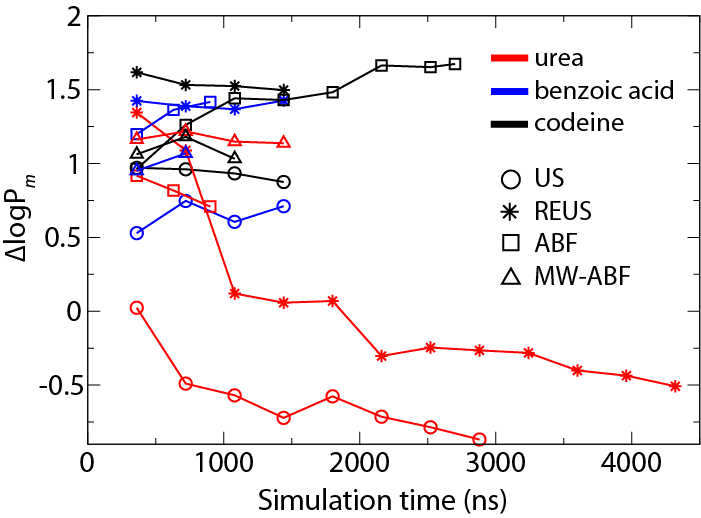
\includegraphics[width=0.65\textwidth]{2015-permeability/Figures/dlogP-recolor.png}
    \caption{ $\Delta$log\perm~of urea (red), benzoic acid (blue) and codeine (black) as a function of simulation time. %For each permeant, $\Delta$log\perm = log\permcom - log\permexp, where log\permcom~and log\permexp~are the computed and experimentally measured log\perm~values, respectively.
    Results obtained with different methods are indicated using the following symbols: US (circle), REUS (star), ABF (square), MW-ABF (triangle). }
    \label{fig:deltaP}
  \end{figure}
